\documentclass[12pt,fleqn,answers]{exam}
\usepackage{amssymb}
\usepackage[intlimits]{amsmath}
\usepackage{epsfig}
\usepackage{upgreek}
\usepackage[super]{nth}
\usepackage[colorlinks=true,linkcolor=black,anchorcolor=black,citecolor=black,filecolor=black,menucolor=black,runcolor=black,urlcolor=black]{hyperref}
\usepackage[letterpaper, margin=0.75in]{geometry}
\addpoints
\boxedpoints
\pointsinmargin
\pointname{pts}
\usepackage{tikz}
\usepackage{tkz-euclide}
\usetikzlibrary{shapes.geometric}
\usetikzlibrary{calc}
\usepackage[final]{microtype}
\frenchspacing
\usepackage[american]{babel}
\usepackage[T1]{fontenc}
\usepackage[]{fourier}
\usepackage{isomath}
\usepackage{upgreek,amsmath}
\usepackage{graphicx}

\newcommand{\dotprod}{\, {\scriptzcriptztyle\stackrel{\bullet}{{}}}\,}

\newcommand{\reals}{\mathbf{R}}
\newcommand{\lub}{\mathrm{lub}} 
\newcommand{\glb}{\mathrm{glb}} 
\newcommand{\complex}{\mathbf{C}}
\newcommand{\dom}{\mbox{dom}}
\newcommand{\range}{\mbox{range}}
\newcommand{\cover}{{\mathcal C}}
\newcommand{\integers}{\mathbf{Z}}
\newcommand{\vi}{\, \mathbf{i}}
\newcommand{\vj}{\, \mathbf{j}}
\newcommand{\vk}{\, \mathbf{k}}
\newcommand{\bi}{\, \mathbf{i}}
\newcommand{\bj}{\, \mathbf{j}}
\newcommand{\bk}{\, \mathbf{k}}
\DeclareMathOperator{\Arg}{\mathrm{Arg}}
\DeclareMathOperator{\Ln}{\mathrm{Ln}}
\newcommand{\imag}{\, \mathrm{i}}

\usepackage{graphicx}
\usepackage{color}
%\shadedsolutions
%\definecolor{SolutionColor}{rgb}{1,0.72,0.46} %{0.8,0.9,1}
\newcommand\AM{\textsc{am}}
\newcommand\PM{\textsc{pm}}
     
\newcommand{\quiz}{13}
\newcommand{\term}{Fall}
\newcommand{\due}{Tuesday October 10 13:20}
\newcommand{\class}{MATH 202, Fall \the\year}
\begin{document}
\large
\vspace{0.1in}
\noindent\makebox[3.0truein][l]{\textbf{\class}}
\textbf{Name:} \hrulefill \\
\noindent \makebox[3.0truein][l]{\textbf{In class work  \quiz}}
\textbf{Row and Seat}:\hrulefill\\

\small
 \noindent   \emph{“Money buys everything except love, personality, freedom, 
    immortality, silence, peace.’’} 
    \hfill \mbox{\sc Carl Sandburg}

    \vspace{0.1in}
\large

\noindent  In class work  \textbf{\quiz}  has questions \textbf{1} 
through  \textbf{\numquestions} \/ with a total of 
\textbf{\numpoints\/}  points. Turn in your work at the end of class 
\emph{on paper}. This assignment is due \emph{\due}.

\vspace{0.1in}

%\normalsize 
\begin{questions} 
    
  \question [2] Use Desmos to graph $y = \sqrt{x^2+1} - x$. Reproduce
  the graph here.  Based on the graph, what is your guess for 
  the numeric value of $\displaystyle \lim_{x \to \infty} \sqrt{x^2+1} - x$?


 
  \begin{solution}[2.5in]
  \vfill
 
    \begin{center}
    %  \begin{figure*}
        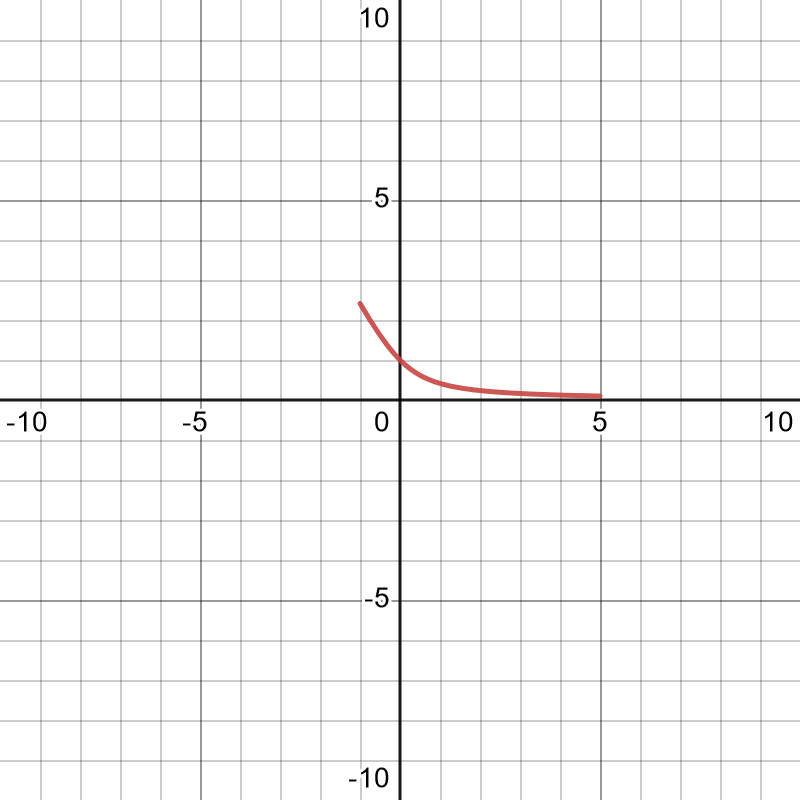
\includegraphics[scale=0.2]{desmos-graph(20).png}
      %\end{figure*}
    \end{center}
    The graph indicates that $\displaystyle \lim_{x \to \infty} \sqrt{x^2+1} - x = 0$. Since $\displaystyle \lim_{x \to \infty} \sqrt{x^2+1} = \infty$
  and \\ \mbox{$\displaystyle \lim_{x \to \infty}  - x = -\infty$}, the limit problem $\displaystyle \lim_{x \to \infty} \sqrt{x^2+1} - x$ gives
an indeterminate form of the type $\infty - \infty$.  

\quad  Knowing that we're dealing with an  indeterminate form of the type $\infty - \infty$ might
tell us something about how to find the limit, but it tells us nothing about the numerical value of the limit.
     \end{solution}

  \question [2] Show that the sequence whose formula is 
  $a_k = \sqrt{k^2+1} - k$ converges. Show all of your work.
  \begin{solution}%[2.5in]
  We'll use the trick of moving the radicals to the denominator. We have
  \begin{align*}
  \lim_{x \to \infty} \sqrt{x^2+1} - x  &= \lim_{x \to \infty} \left(\sqrt{x^2+1} - x \right)   \times \frac{\sqrt{x^2+1}  + x}{\sqrt{x^2+1}  + x}, \\
                                                                 &= \lim_{x \to \infty} \frac{(x^2+1) - x^2}{\sqrt{x^2+1}  + x}, \\
                                                                 &=  \lim_{x \to \infty} \frac{1}{\sqrt{x^2+1}  + x}, \\
      \intertext{We have $\displaystyle \lim_{x \to \infty}    \sqrt{x^2+1}  + x = \infty$, so we have}                                                        
                                                                 &=  0
  \end{align*}
  Although the calculation $\displaystyle \lim_{x \to \infty} \frac{1}{\sqrt{x^2+1}  + x} = \frac{1}{\infty} = 0$ is based on a theorem, it's not considered   to be something you should do in public. Specifically, the theorem is: If $\displaystyle \lim_a   F \in \reals$ and $\displaystyle \lim_a G \in \reals = \infty$,
  then $\displaystyle \lim_a \frac{F}{G} = 0$. Be careful with this--the limit of the numerator must be a real number.
  \end{solution}

  \newpage
  \question [2] Determine if the sequence whose formula is 
  $b_k = k \ln \left(1+\frac{8}{k} \right)$ converges. If it does, find its 
  limit. As always, show your work.
  \begin{solution}%[2.5in]
We need the limit of a product. Since $\displaystyle \lim_{k \to \infty} k = \infty$ and $\displaystyle \lim_{k \to \infty} \left(1+\frac{8}{k} \right) = 0$, we have an indeterminate form of the type $0 \times \infty$. By rearranging this to $\frac{\left(1+\frac{8}{k} \right) }{\frac{1}{k}}$,
we have an  indeterminate form of the type $\frac{0}{0}$. And maybe the l'Hôpital rule will help.  We have
\begin{align*}
  \lim_{ k  \to \infty} \ln \left(1+\frac{8}{k} \right) &=  \lim_{k \to \infty} \frac{\left(1+\frac{8}{k} \right) }{\frac{1}{k}}, \\
                                                                                          &= \lim_{k \to \infty} \frac{ -\frac{8}{\left( \frac{8}{k}+1\right) \, {{k}^{2}}}}{-\frac{1}{k^2}}\\
                                                                                          &=  \lim_{k \to \infty} \frac{8}{\frac{8}{k}+1}, \\
                                                                                          &= 8.
\end{align*}
  Actually, until we've determined that the limit of the quotient of derivatives is a real number, equality between the first and second lines is 
  not certain.  Notionally, we could use $\overset{?}{=}$ To mean equality as long as the right side is a real number, but that notation (I didn't invent it) is a bit weird.
  \end{solution}

  \newpage
  \question A sequence $c$ is defined recursively by
  \begin{equation*}
      c_n = \begin{cases} 2 & n=0 \\
                          5 & n=1 \\
                          5 c_{n-1}-6 c_{n-2} & n=2,3,4,\dots
      \end{cases}
    \end{equation*}
        
\begin{parts}
\part[2] Find the numeric values of $c_2, c_3$, and $c_4$.
\begin{solution}[2.5in]
\begin{align*}
   c_2 &= 5 c_1 - 6 c_0 = 5 \times  5 - 6 \times 2 = 25-12 = 13,\\
   c_3 &= 5 c_2 - 6 c_1 = 5 \times  13 - 6 \times 5 = 65-30 = 35,\\
    c_4 &= 5 c_3 - 6 c_2 = 5 \times  35 - 6 \times 13= 25-12 = 97.
\end{align*}
\end{solution}

\part [2] Show that $c_n = 2^n +3^n$ is a solution to the equation
$c_n = 5 c_{n-1}-6 c_{n-2}$. To do this, show that 
$c_n = 5 c_{n-1}-6 c_{n-2}$ simplifies to an identity using
$c_n = 2^n +3^n$.
\end{parts}
\begin{solution}[2.5in] We have
\begin{align*}
  \left[ c_n = 5 c_{n-1}-6 c_{n-2} \right] &= \left[  2^n +3^n = 5 ( 2^{n-1} +3^{n-1}) - 6 (  2^{n-2} +3^{n-2} ) \right], \\
                                                                      &=  \left[  2^n +3^n = \frac{5}{2}  \times  2^{n} + \frac{3}{2} \times 3^{n} - \frac{6}{4}   \times 2^n + \frac{6}{9} \times 3^n \right],\\
              &=\left[  2^n +3^n = 2^n +3^n     \right], \\
              &= \text{True}.                                                    
\end{align*}
\end{solution}

  \end{questions}
\end{document}

